\documentclass[tikz,border=8pt]{standalone}
% Shared look for every TikZ diagram. Load with \input{../../tools/tikz-style.tex}
\usepackage[T1]{fontenc}
\usepackage{lmodern}
\renewcommand{\sfdefault}{lmr}  % diagrams use the same serif as the text
\usetikzlibrary{arrows.meta, positioning, shapes.geometric, calc, fit, backgrounds}
\definecolor{cblue}{HTML}{4C78A8}
\definecolor{corange}{HTML}{F58518}
\definecolor{cgreen}{HTML}{54A24B}
\definecolor{cred}{HTML}{E45756}
\definecolor{cpurple}{HTML}{B279A2}
\definecolor{cgrey}{HTML}{6B6B6B}
\tikzset{
  every picture/.style={font=\sffamily, line width=1.2pt},
  box/.style={draw=#1, fill=#1!12, rounded corners=4pt, align=center, inner sep=7pt, minimum height=1.1cm},
  box/.default=cgrey,
  arrow/.style={-{Stealth[length=3mm]}, draw=cgrey, line width=1.4pt},
  title/.style={font=\sffamily\bfseries\Large},
  note/.style={font=\sffamily\small, text=cgrey, align=center},
}
\AtBeginDocument{\hyphenpenalty=10000 \exhyphenpenalty=10000}

\begin{document}
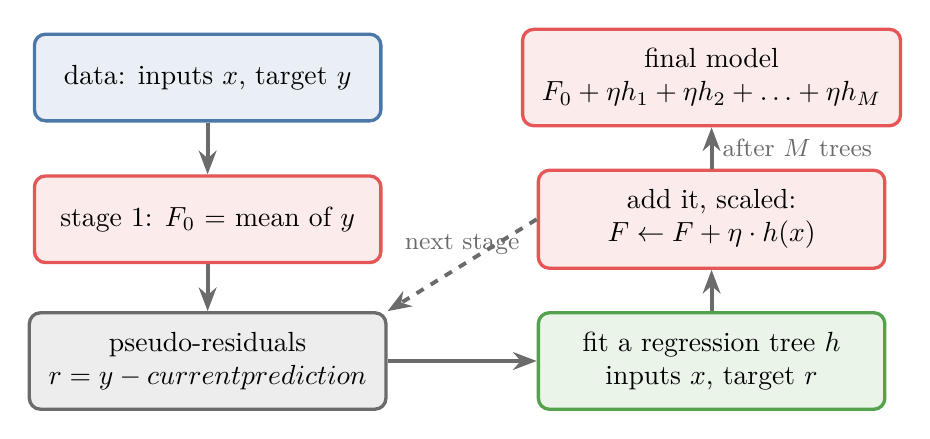
\begin{tikzpicture}[b/.style={box=cblue, minimum width=4.4cm}, g/.style={box=cgrey, minimum width=4.4cm},
  r/.style={box=cred, minimum width=4.4cm}, gr/.style={box=cgreen, minimum width=4.4cm}]
  \node[b] (data) at (0,0) {data: inputs $x$, target $y$};
  \node[r] (f0) at (0,-1.8) {stage 1: $F_0$ = mean of $y$};
  \node[g] (res) at (0,-3.6) {pseudo-residuals\\$r = y - \text{current prediction}$};
  \node[gr] (tree) at (6.4,-3.6) {fit a regression tree $h$\\inputs $x$, target $r$};
  \node[r] (upd) at (6.4,-1.8) {add it, scaled:\\$F \leftarrow F + \eta \cdot h(x)$};
  \node[r] (out) at (6.4,0) {final model\\$F_0 + \eta h_1 + \eta h_2 + \dots + \eta h_M$};
  \draw[arrow] (data) -- (f0); \draw[arrow] (f0) -- (res); \draw[arrow] (res) -- (tree);
  \draw[arrow] (tree) -- (upd);
  \draw[arrow, dashed] (upd.west) -- node[note, above] {next stage} (res.north east);
  \draw[arrow] (upd) -- node[note, right] {after $M$ trees} (out);
\end{tikzpicture}
\end{document}
